\documentclass[a4paper,11pt]{article}
\input{/home/tof/Documents/Cozy/latex-include/preambule_lua.tex}
\newcommand{\showprof}{show them}  % comment this line if you don't want to see todo environment
\fancyhead[L]{Carte d'orientation - représentation}
\newdate{madate}{10}{09}{2020}
\fancyhead[R]{Terminale - NSI} %\today
\fancyfoot[L]{~\\Christophe Viroulaud}
\AtEndDocument{\label{lastpage}}
\fancyfoot[C]{\textbf{Page \thepage/\pageref{lastpage}}}
\fancyfoot[R]{\includegraphics[width=2cm,align=t]{/home/tof/Documents/Cozy/latex-include/cc.png}}
\usepackage{tikz}
\begin{document}
\begin{Form}
\begin{commentprof}
mettre \textbf{carte\_co.zip} sur site; donner d'abord les pages 1, 2 seulement
\end{commentprof}
\section{Problématique}
La \emph{course d'orientation} est une activité proposée par l'association sportive du lycée. C'est un sport très complet et apprécié des élèves. Cependant un inconvénient pour les enseignants qui organisent une séance est le temps de préparation nécessaire. Un support numérique peut permettre d'optimiser ce temps.
\begin{center}
\begin{tabular}{cc}
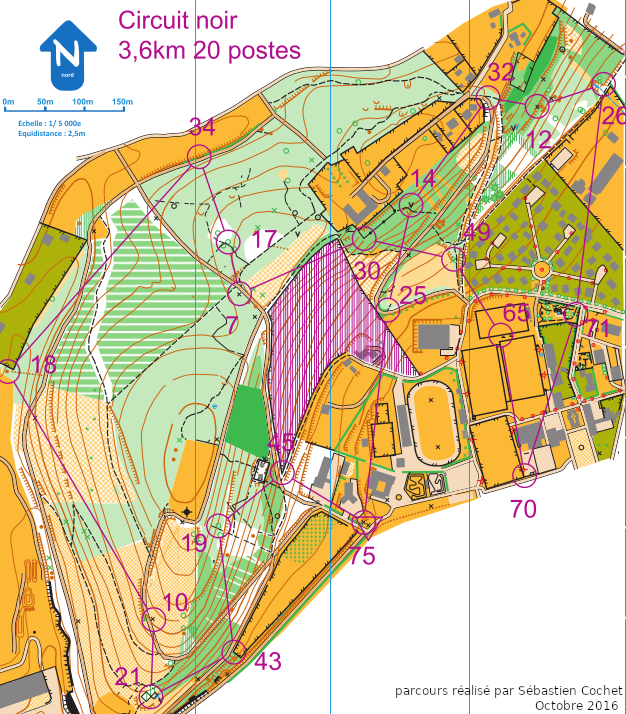
\includegraphics[width=7.5cm]{ressources/co-noir.png}
  & 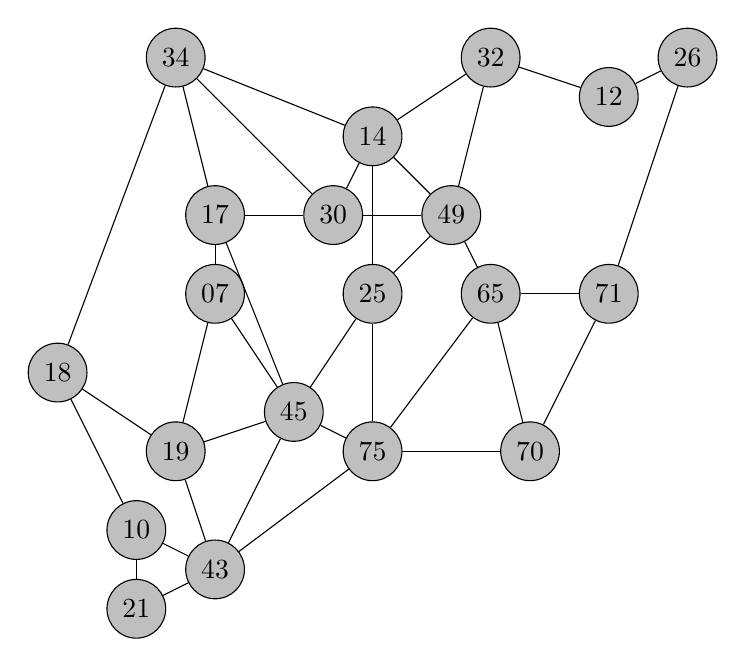
\begin{tikzpicture}
\node[draw,circle,fill=gray!50] (21)at(0,0) {21};
\node[draw,circle,fill=gray!50] (43)at(1,0.5) {43};
\node[draw,circle,fill=gray!50] (10)at(0,1) {10};
\node[draw,circle,fill=gray!50] (19)at(0.5,2) {19};
\node[draw,circle,fill=gray!50] (45)at(2,2.5) {45};
\node[draw,circle,fill=gray!50] (18)at(-1,3) {18};
\node[draw,circle,fill=gray!50] (75)at(3,2) {75};
\node[draw,circle,fill=gray!50] (70)at(5,2) {70};
\node[draw,circle,fill=gray!50] (65)at(4.5,4) {65};
\node[draw,circle,fill=gray!50] (71)at(6,4) {71};
\node[draw,circle,fill=gray!50] (25)at(3,4) {25};
\node[draw,circle,fill=gray!50] (07)at(1,4) {07};
\node[draw,circle,fill=gray!50] (17)at(1,5) {17};
\node[draw,circle,fill=gray!50] (30)at(2.5,5) {30};
\node[draw,circle,fill=gray!50] (49)at(4,5) {49};
\node[draw,circle,fill=gray!50] (14)at(3,6) {14};
\node[draw,circle,fill=gray!50] (34)at(0.5,7) {34};
\node[draw,circle,fill=gray!50] (32)at(4.5,7) {32};
\node[draw,circle,fill=gray!50] (12)at(6,6.5) {12};
\node[draw,circle,fill=gray!50] (26)at(7,7) {26};

\draw[-,>=latex] (75) -- (45);
\draw[-,>=latex] (75) -- (25);
\draw[-,>=latex] (75) -- (65);
\draw[-,>=latex] (75) -- (70);
\draw[-,>=latex] (75) -- (43);
\draw[-,>=latex] (45) -- (07);
\draw[-,>=latex] (45) -- (43);
\draw[-,>=latex] (45) -- (25);
\draw[-,>=latex] (45) -- (19);
\draw[-,>=latex] (45) -- (17);
\draw[-,>=latex] (25) -- (14);
%\draw[-,>=latex] (19) -- (10);
\draw[-,>=latex] (19) -- (18);
\draw[-,>=latex] (19) -- (07);
\draw[-,>=latex] (19) -- (43);
\draw[-,>=latex] (43) -- (10);
\draw[-,>=latex] (43) -- (21);
%\draw[-,>=latex] (43) -- (18);
\draw[-,>=latex] (10) -- (21);
\draw[-,>=latex] (10) -- (18);
\draw[-,>=latex] (34) -- (17);
\draw[-,>=latex] (70) -- (71);
\draw[-,>=latex] (70) -- (65);
\draw[-,>=latex] (49) -- (65);
\draw[-,>=latex] (49) -- (25);
\draw[-,>=latex] (49) -- (14);
\draw[-,>=latex] (49) -- (30);
\draw[-,>=latex] (49) -- (32);
\draw[-,>=latex] (30) -- (14);
\draw[-,>=latex] (30) -- (34);
\draw[-,>=latex] (30) -- (17);
\draw[-,>=latex] (14) -- (34);
\draw[-,>=latex] (14) -- (32);
\draw[-,>=latex] (32) -- (12);
\draw[-,>=latex] (12) -- (26);
\draw[-,>=latex] (65) -- (71);
\draw[-,>=latex] (71) -- (26);
\draw[-,>=latex] (18) -- (34);
\draw[-,>=latex] (07) -- (17);

\end{tikzpicture} \\ 
\end{tabular} 
\captionof{figure}{Parcours noir}
\label{co}
\end{center}

\begin{center}
\shadowbox{\parbox{12cm}{\centering Comment peut-on représenter les balises de CO en mémoire ?}}
\end{center}
\section{Notion de graphe}
Un graphe est l'ensemble des \textbf{sommets} et des \textbf{arêtes} qui relient certains sommets entre eux. L'\textbf{ordre} du graphe est le nombre de sommets. Le \textbf{degré d'un sommet} est le nombre d'arêtes de ce sommet. Deux sommets reliés entre eux sont dits \textbf{adjacents}. Enfin un graphe est dit \textbf{complet} si tous les sommets sont adjacents.
\begin{activite}
\begin{enumerate}
\item Donner le degré du sommet 30.
\item Donner deux sommets adjacents.
\item Donner l'ordre et la somme des degrés du graphe figure \ref{co}.
\item Ce graphe est-il complet?
\item Schématiser un graphe complet d'ordre 4.
\end{enumerate}
\end{activite}
\section{Représentations en mémoire}
\subsection{Matrice d'adjacence}
On appelle \textbf{matrice d'adjacence} la représentation mathématique dont le terme $a_{ij}$ vaut 1 si les sommets \emph{i} et \emph{j} sont reliés par une arête et 0 sinon.

\begin{figure}[!h]
\centering
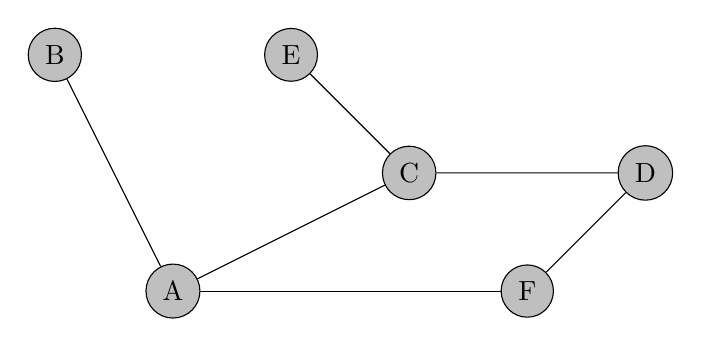
\begin{tikzpicture}[scale=1.5]
\node[draw,circle,fill=gray!50] (A)at(0,0) {A};
\node[draw,circle,fill=gray!50] (B)at(-1,2) {B};
\node[draw,circle,fill=gray!50] (C)at(2,1) {C};
\node[draw,circle,fill=gray!50] (D)at(4,1) {D};
\node[draw,circle,fill=gray!50] (E)at(1,2) {E};
\node[draw,circle,fill=gray!50] (F)at(3,0) {F};
\draw[-,>=latex] (A) -- (B);
\draw[-,>=latex] (A) -- (C);
\draw[-,>=latex] (A) -- (F);
\draw[-,>=latex] (C) -- (E);
\draw[-,>=latex] (C) -- (D);
\draw[-,>=latex] (D) -- (F);
\end{tikzpicture}
\captionof{figure}{Graphe étudié}
\label{graphe0}
\end{figure}

La matrice d'adjacence du graphe \ref{graphe0} est:
$$\begin{pmatrix}
0 & 1 & 1 & 0 & 0 & 1 \\
1 & 0 & 0 & 0 & 0 & 0 \\
1 & 0 & 0 & 1 & 1 & 0 \\
0 & 0 & 1 & 0 & 0 & 1 \\
0 & 0 & 1 & 0 & 0 & 0 \\
1 & 0 & 0 & 1 & 0 & 0 \\
\end{pmatrix}$$
\begin{activite}
Déterminer une structure de données permettant de représenter la matrice d'adjacence en mémoire.
\end{activite}
On notera la symétrie dans la matrice. Cette observation s'explique aisément: L'arête de A vers B est également représentée par celle de B vers A.\\
Cette représentation est relativement simple à utiliser mais n'est pas toujours économe en ressource mémoire, particulièrement si le nombre d'arêtes est faible: la matrice sera \emph{creuse}.
\subsection{Dictionnaire d'adjacence}
Une autre terminologie consiste à, pour chaque sommet, énumérer les sommets adjacents: c'est le \textbf{dictionnaire d'adjacence}.
\begin{itemize}
\item A: B, C, F
\item B: A
\item C: A, D, E
\item D: C, F
\item E: C
\item F: A, D
\end{itemize}
\begin{activite}
Construire le dictionnaire d'adjacence en mémoire.
\end{activite}
\begin{commentprof}
littérature: existe aussi liste d'adjacence, liste successeur...\\
pour stocker les nœuds successeurs on peut utiliser une liste ou mieux un set: collection non triée d'objets distincts
\end{commentprof}
Cette représentation aura notre préférence. Contrairement à la matrice d'adjacence, il n'est pas nécessaire de connaître touts les sommets à l'avance pour la construire. De plus, à part pour les cas où pratiquement tous les sommets sont reliés entre eux, elle occupe moins d'espace.
\subsection{Représentation de la carte de CO}
Appliquons ces représentations à la carte de CO. 
\begin{activite}
\begin{enumerate}
\item Représenter en mémoire la matrice d'adjacence et le dictionnaire d'adjacence de la carte (figure \ref{co}).
\item Récupérer le dossier compressé \textbf{carte\_co.zip} sur le site \url{htps://cviroulaud.github.io}
\item Importer la bibliothèque \textbf{mod\_verification} et utiliser la fonction \textbf{verifier(graphe)}.
\end{enumerate}
\end{activite}
\section{Utilisation de la programmation objet}
Les graphes trouvent de multiples applications dans de nombreux domaines. Il ne paraît alors pas inutile de créer une classe générique que nous pourrons utiliser dans des situations différentes.\\
Nous préférerons l'utilisation d'un dictionnaire d'adjacence pour contenir les sommets.
\begin{activite}
\begin{enumerate}
\item Créer une classe \textbf{Graphe}. Elle possédera un attribut \textbf{sommets}, dictionnaire vide.
\item Créer la méthode \textbf{ajouter\_sommet(self, s)$\;\rightarrow\;$None} qui crée la clé \emph{s} dans \emph{sommets}. La valeur correspondante sera un \emph{set} vide. Cette méthode vérifiera si le sommet n'est pas déjà présent avant de l'ajouter.\\Il faut noter que le paramètre \emph{s} est un entier dans le cas de notre carte de CO mais nous pourrions avoir une chaîne de caractère ou même d'autres structures plus complexes.
\item Créer la méthode \textbf{ajouter\_arete(self, s1, s2)$\;\rightarrow\;$None} qui:
\begin{itemize}
\item ajoute les sommets s'ils ne sont pas déjà présents,
\item crée les arêtes entre les deux sommets.
\end{itemize}
\item Créer la méthode \textbf{sont\_relies(self, s1, s2)$\;\rightarrow\;$bool} qui renvoie \emph{True} s'il existe une arête entre s1 et s2.
\item Créer la méthode \textbf{get\_adjacents(self, s)$\;\rightarrow\;$set} qui renvoie les sommets voisins de \emph{s}.
\item Créer la méthode \textbf{get\_sommets(self)$\;\rightarrow\;$list} qui renvoie la liste des sommets.
\item Créer une instance \textbf{parcours\_noir} de la classe Graphe.\\
Le fichier \emph{parcours\_noir.json} contient la structure du parcours. Ce type de fichier permet de stocker des données facilement. Python gère ce format avec la bibliothèque \emph{json}. Les accolades sont transformées en dictionnaire et les crochets en liste.
\item Observer la structure des données dans le fichier \emph{json}.
\item Importer le fichier en lecture dans le programme Python et remplir l'instance \emph{parcours\_noir} du \emph{Graphe}. La méthode \emph{load} de la bibliothèque \emph{json} est suffisante.
\end{enumerate}
\end{activite}
\begin{commentprof}
pour les clés, il faut une structure non mutable (donc hashable)\\
on utilisera set() plutôt que list() car pour des grands graphes, set sera plus efficace\\
list(dictionnaire) renvoie la liste des clés

\end{commentprof}
\end{Form}
\end{document}